\subsection{Ví Dụ R: Dataset \texttt{Boston}}
% -----------------------------------------------------------------------------

\textbf{Bài toán.} Dự báo giá trị nhà trung vị (\texttt{medv}) từ tỷ lệ dân cư thu nhập thấp (\texttt{lstat}) và số phòng trung bình (\texttt{rm}):
\[
  \texttt{medv} = \beta_0 + \beta_1\texttt{lstat} + \beta_2\texttt{rm} + \varepsilon.
\]

Mục tiêu của ví dụ này không chỉ là kiểm tra xem phần dư có chuẩn hay không. Với $n=506$, các kiểm định chuẩn tắc rất dễ bác bỏ $H_0$. Câu hỏi thực hành quan trọng hơn là: \textbf{kết luận về hệ số có ổn định khi thay suy diễn OLS cổ điển bằng HC3 và bootstrap hay không?}

\subsubsection*{Bước 1: Fit mô hình và vẽ chẩn đoán}

\begin{lstlisting}[style=Rstyle]
library(MASS)
data(Boston)

model_boston <- lm(medv ~ lstat + rm, data = Boston)
resid_raw    <- residuals(model_boston)
resid_stud   <- rstudent(model_boston)
\end{lstlisting}

\begin{figure}[H]
  \centering
  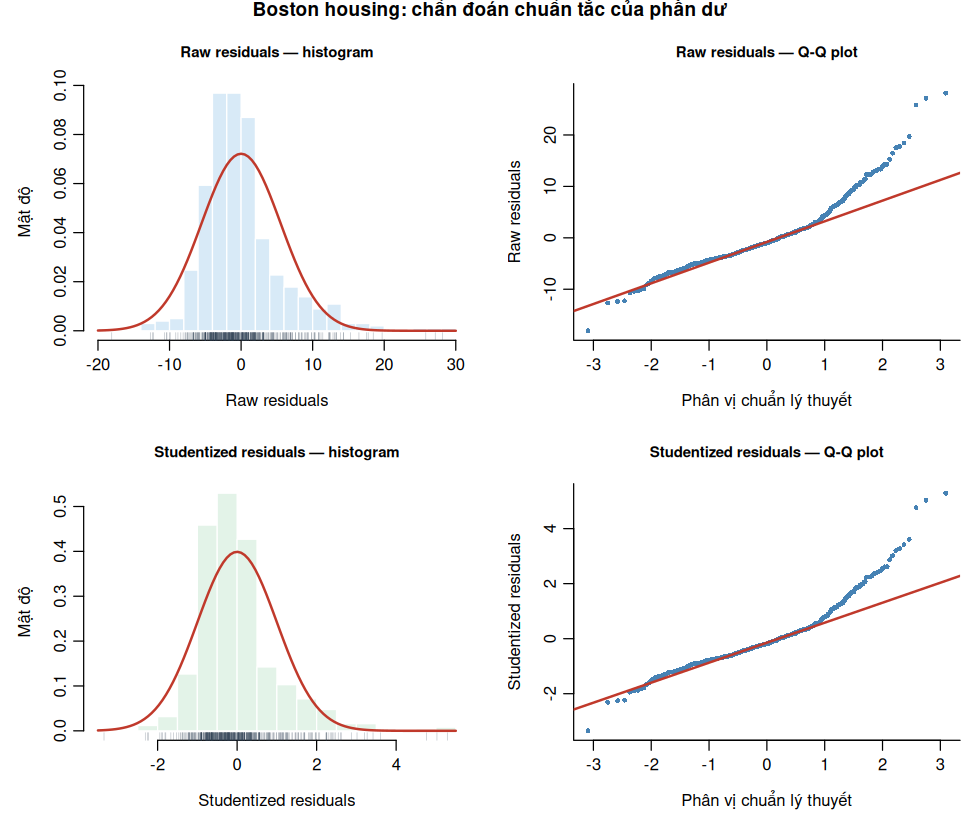
\includegraphics[width=\textwidth]{./figures/fig17_boston_normality.png}
  \caption{Chẩn đoán chuẩn tắc cho mô hình \texttt{medv \textasciitilde{} lstat + rm}. Hàng trên dùng raw residuals; hàng dưới dùng phần dư Student hóa ngoài. Cả hai Q-Q plot đều cho thấy đuôi phải lệch mạnh khỏi đường chuẩn, tức có một số giá trị nhà được dự báo thấp hơn thực tế khá nhiều.}
  \label{fig:boston_normality}
\end{figure}

\textbf{Quan sát.} Histogram và Q-Q plot đều cho thấy phần dư lệch phải và có đuôi dày. Phần dư Student hóa làm tín hiệu ở đuôi rõ hơn vì đã điều chỉnh phương sai phần dư theo leverage.

\subsubsection*{Bước 2: Kiểm định hình thức}

\begin{lstlisting}[style=Rstyle]
shapiro.test(resid_raw)

# Jarque-Bera tinh thu cong: skewness + excess kurtosis
n  <- length(resid_raw)
z  <- resid_raw - mean(resid_raw)
m2 <- mean(z^2)
S  <- mean(z^3) / m2^(3/2)
K  <- mean(z^4) / m2^2 - 3
JB <- n / 6 * (S^2 + K^2 / 4)
pchisq(JB, df = 2, lower.tail = FALSE)
\end{lstlisting}

\begin{lstlisting}[style=output]
Shapiro-Wilk: W = 0.9098, p-value < 2.2e-16
Jarque-Bera : JB = 457.6899, p-value = 4.11e-100
Skewness    : S = 1.3432
Excess kurt.: K = 3.8068
\end{lstlisting}

Cả hai kiểm định đều bác bỏ chuẩn tắc rất mạnh. Với $n=506$, điều này không bất ngờ: kiểm định có power lớn và phát hiện được cả những sai lệch nhỏ. Ở đây sai lệch không chỉ nhỏ; Q-Q plot cho thấy đuôi phải rõ ràng. Vì vậy, ta chuyển sang kiểm tra độ nhạy của suy diễn hệ số.

\subsubsection*{Bước 3: OLS SE, HC3 SE và Bootstrap CI}

Đoạn code sau tính HC3 thủ công để không phụ thuộc vào package ngoài. Ý tưởng là giữ nguyên hệ số OLS, nhưng thay ma trận hiệp phương sai cổ điển bằng sandwich estimator có hiệu chỉnh leverage.

\begin{lstlisting}[style=Rstyle]
X       <- model.matrix(model_boston)
e       <- residuals(model_boston)
h       <- hatvalues(model_boston)
XtX_inv <- solve(t(X) %*% X)

meat <- t(X) %*% diag(as.numeric(e^2 / (1 - h)^2)) %*% X
V_hc3 <- XtX_inv %*% meat %*% XtX_inv
se_hc3 <- sqrt(diag(V_hc3))

# Case bootstrap cho he so
library(boot)
boot_fn <- function(data, indices) {
  coef(lm(medv ~ lstat + rm, data = data[indices, ]))
}
set.seed(123)
boot_out <- boot(Boston, boot_fn, R = 2000)
\end{lstlisting}

\begin{center}
\scriptsize
\begin{tabularx}{\textwidth}{@{}lrrrr>{\raggedright\arraybackslash}X>{\raggedright\arraybackslash}X@{}}
\toprule
\textbf{Biến} & \textbf{Estimate} & \textbf{OLS SE} & \textbf{HC3 SE} & \textbf{Tỷ lệ} & \textbf{OLS 95\% CI} & \textbf{Bootstrap 95\% CI} \\
\midrule
\texttt{lstat} & $-0.6424$ & $0.0437$ & $0.0654$ & $1.50$ & $[-0.7283, -0.5564]$ & $[-0.7628, -0.5152]$ \\
\texttt{rm}    & $ 5.0948$ & $0.4445$ & $0.7939$ & $1.79$ & $[4.2216, 5.9680]$ & $[3.5423, 6.5887]$ \\
\bottomrule
\end{tabularx}
\end{center}

\textbf{Diễn giải.} HC3 SE lớn hơn OLS SE khá rõ: khoảng $1.5$ lần cho \texttt{lstat} và $1.79$ lần cho \texttt{rm}. Bootstrap CI cũng rộng hơn OLS CI và khá gần với suy diễn robust. Tuy vậy, dấu và độ lớn thực hành của hai hệ số vẫn ổn định: \texttt{lstat} có quan hệ âm với \texttt{medv}, còn \texttt{rm} có quan hệ dương.

\subsubsection*{Bước 4: Kiểm tra ảnh hưởng}

\begin{lstlisting}[style=Rstyle]
max(abs(rstudent(model_boston)))
max(cooks.distance(model_boston))
max(hatvalues(model_boston))
\end{lstlisting}

\begin{lstlisting}[style=output]
max |rstudent| = 5.2869
max Cook's D   = 0.2566
max leverage   = 0.0633
\end{lstlisting}

Có phần dư Student hóa rất lớn, nên đuôi phải trên Q-Q plot không chỉ là chi tiết hình thức. Tuy nhiên, leverage lớn nhất không quá cao trong mô hình hai biến này. Workflow hợp lý là báo cáo suy diễn robust/bootstrap và, nếu đây là phân tích chính thức, kiểm tra thêm các quan sát có Cook's distance lớn hoặc cân nhắc biến đổi/mô hình linh hoạt hơn.

\subsubsection*{Kết Luận Ví Dụ}

\begin{notebox}
\textbf{Bài học từ Boston.} Kiểm định chuẩn tắc bác bỏ rất mạnh, nhưng kết luận không phải là ``vứt mô hình OLS''. Với $n=506$, cần nhìn vào độ nhạy của suy diễn: HC3 và bootstrap làm khoảng tin cậy rộng hơn đáng kể, nhưng không đổi kết luận định tính về \texttt{lstat} và \texttt{rm}. Vì vậy, báo cáo tốt hơn là: mô hình OLS cho xu hướng rõ ràng, nhưng suy diễn nên dùng robust SE hoặc bootstrap CI thay vì chỉ dựa vào SE cổ điển.
\end{notebox}

% -----------------------------------------------------------------------------
